\section{Subdivision}

We will begin the proof of the locality principle today, 
and finish it in the next lecture.
The key is a process of subdivision of singular simplices. It will use the 
``cone construction'' $b*$ from Lecture 5. The cone construction 
dealt with a region $X$ 
in Euclidean space, star-shaped with respect to $b\in X$, and gave a 
chain-homotopy between the identity and the ``constant map'' on $S_*(X)$:
\[
db*+b*d=1-\eta\epsilon
\]
where $\epsilon:S_*(X)\to\ZZ$ is the augmentation and $\eta:\ZZ\to S_*(X)$
sends 1 to the constant 0-chain $c_b^0$. 

Let's see how the cone construction can be used to ``subdivide'' an ``affine 
simplex.'' An {\em affine simplex} is the convex hull of a finite set of points in Euclidean space. To make this non-degenerate, assume that the points $v_0,v_1,\ldots,v_n$, have the property that $\{v_1-v_0,\ldots,v_n-b_0\}$ is linearly independent. 
The {\em barycenter} of this simplex is the center of mass of the vertices, 
\[
b=\frac{1}{n+1}\sum{v_i}\,.
\]

Start with $n=1$. To subdivide a 1-simplex, just cut it in half. 
For the $2$-simplex, look at the subdivision of each face, and form the cone
of them with the barycenter of the 2-simplex. This gives us a decomposition of
the 2-simplex into six sub-simplices. 

\begin{center}
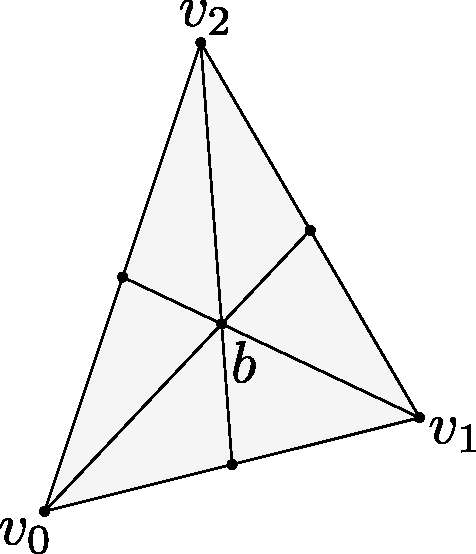
\includegraphics[width=3in]{905/Figures/12-subdivision.pdf}
\end{center}

We want to formalize this process, and extend it to singular simplices (using
naturality, of course). Define a natural transformation 
\[
\$:S_n(X)\to S_n(X)
\]
 by defining it on standard $n$-simplex, namely by specifying what $\$(\iota_n)$ is where $\iota_n:\Delta^n\rightarrow\Delta^n$ is the universal $n$-simplex, and then extending by naturality:
\[
\$(\sigma)=\sigma_\ast\$(\iota_n)\,.
\]
Here's the definition. When $n=0$, define $\$$ to be the identity; i.e., $\$\iota_0=\iota_0$. For $n>0$, define 
\[
\$\iota_n:=b_n\ast\$ d\iota_n
\]
where $b_n$ is the barycenter of $\Delta^n$. This makes a \emph{lot} of sense if you draw out a picture, and it's a very clever definition that captures the geometry we described. Here's what we'll prove.
\begin{prop}
$\$$ is a natural chain map $S_\ast(X)\to S_\ast(X)$ that is naturally chain-homotopic to the identity. 
\end{prop}

\noindent
\begin{proof}
Let's try to prove that it's a chain map. We'll use induction on $n$. It's enough to show that $d\$\iota_n=\$ d\iota_n$, because then, for any $n$-simplex $\sigma$,
$$
d\$\sigma=d\$\sigma_\ast\iota_n=\sigma_\ast d\$\iota_n=\sigma_\ast \$d\iota_n=\$ d\sigma_\ast\iota_n=\$ d\sigma\,.
$$

Dimension zero is easy:
since $S_{-1}=0$, $d\$\iota_0$ and $\$d\iota_0$ are both zero and hence equal.

For $n\geq 1$, we want to compute $d\$\iota_n$. This is:
\begin{align*}
d\$\iota_n & =d(b_n\ast \$ d\iota_n)  \\
 & = (1-\eta_b\epsilon-b_n\ast d)(\$ d\iota_n)
\end{align*}
What happens when $n=1$? Well,
$$
\eta_b\epsilon\$d\iota_1 = \eta_b\epsilon \$(c^0_1 - c^0_0)=\eta_b\epsilon(c^0_1 - c^0_0)=0\,,
$$
since $\epsilon$ takes sums of coefficients. So the $\eta_b\epsilon$ term drops out for any $n\geq1$. Let's continue, using the inductive hypothesis:
\begin{align*}
d\$\iota_n & = (1 - b_n\ast d)(\$ d\iota_n) \\
 & = \$d\iota_n - b_n\ast d\$ d\iota_n  \\
 & = \$d\iota_n - b_n\$d^2\iota_n &\\
 & = \$d\iota_n 
\end{align*}
because $d^2=0$. 

To define the chain homotopy $T$, we'll just write down a formula and not try to justify it. Making use of naturality, we just need to define $T\iota_n$. 
Here it is:
\[
T\iota_n = b_n\ast(\$\iota_n - \iota_n - Td\iota_n)\in S_{n+1}(\Delta^n) \,.
\]
Once again, we're going to check that $T$ is a chain homotopy by induction, and, again, we need to check only on the universal case.

When $n=0$, the formula gives $T\iota_0=0$, so it's true that $dT\iota_0-Td\iota_0=\$\iota_0-\iota_0$.
Now let's assume that $dTc-Tdc=\$c-c$ for every $(n-1)$-chain. Let's start by computing $dT\iota_n$:
\begin{align*}
dT\iota_n & = d_n(b_n\ast(\$\iota_n - \iota_n - Td\iota_n)) \\
& = (1-b_n\ast d)(\$\iota_n - \iota_n - Td\iota_n) \\
& = \$\iota_n-\iota_n-Td\iota_n-b_n\ast (d\$\iota_n - d\iota_n - dTd\iota_n)
\end{align*}
All we want now is that $b_n\ast(d\$\iota_n - d\iota_n - dTd\iota_n)=0$. We can do this using the inductive hypothesis, because $d\iota_n$ is in dimension $n-1$.
\begin{align*}
dTd\iota_n & = -Td(d\iota_n)+\$ d\iota_n - d\iota_n\\
& = \$d\iota_n - d\iota_n\\
& = d\$\iota_n - d\iota_n\,.
\end{align*}
This means that $d\$\iota_n-d\iota_n - dTd\iota_n=0$, so $T$ is indeed a chain homotopy. 
\end{proof}
